\section*{Question 4}

The next contribution to the while language, is the binary disjunction on booleans. This new operator again calls for a new class \texttt{OrExpr} similar to the supplied \texttt{AndExpr} class. The only difference, is the use of '$||$' instead of '$\&\&$' in the \texttt{evaluate} method. 


When working with booleans, just like arithmetic, we want to have a clear sense of hierarchy when operators are executed. The hierarchy here is: negation, conjunction and disjunction, in order from strongest to weakest binding. To implement this in the while language, we introduce a new rule, to make sure that the conjunction is evaluated before the disjunction (effectively moving it a step down in the parse tree). The negation is implemented in the \texttt{literal} rule (which is even further down the parse tree). This is seen in the code snippet below:

\begin{lstlisting}
bool_expr returns [BoolExpr value]
  : e=conj_bool_expr  { $value = e; }
  //Added conj_bool_expr to maintain hierachy
  ('||' e=conj_bool_expr  { $value = new OrExpr($value,e);})*
;

//Binds stronger than disjunc operator
conj_bool_expr returns [BoolExpr value]
  : e=literal   { $value = e; }
  ('&&' e=literal    { $value = new AndExpr($value,e);})*
;

//Binds stronger than conjunc operator
literal returns [BoolExpr value]
  : e=base_bool_expr  { $value = e; }
  | '!' e=literal { $value = new NotExpr(e); }
;
\end{lstlisting}

The hierarchy is shown to be correct in figure \ref{fig:Q4ex}

\begin{figure}[H]
    \centering
    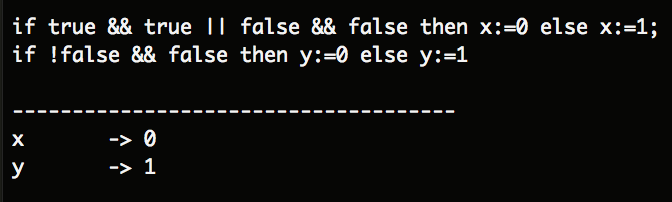
\includegraphics[width=0.6\textwidth]{fig/Q4example}
    \caption{Example of hierarchy for negation, conjunction and disjunction operators with correct answers: x = 0 and y = 1.}
    \label{fig:Q4ex}
\end{figure}

For the first if statement of the example shown in figure \ref{fig:Q4ex}, the expression can be evaluated as seen in figure \ref{fig:Q4hierarchy}. This figure shows, that with conjunction binding stronger than disjunction, the correct answer for the first if-statement is x = 0.

\begin{figure}[H]
\begin{subfigure}{0.49\textwidth}
\begin{gather*}
     \text{true \&\& true $||$ false \&\& false} \Rightarrow\\
     \text{true \&\& true \&\& false} \Rightarrow\\
     \text{true \&\& false} \Rightarrow\\
     \text{false}
\end{gather*}
\vspace{-7mm}
\caption{}
\label{fig:dis}
\end{subfigure}
\begin{subfigure}{0.49\textwidth}
\begin{gather*}
     \text{true \&\& true $||$ false \&\& false} \Rightarrow\\
     \text{true $||$ false \&\& false} \Rightarrow\\
     \text{true $||$ false} \Rightarrow\\
     \text{true}
\end{gather*}
\vspace{-7mm}
\caption{}
\label{fig:con}
\end{subfigure}
 
\caption{Evaluating condition with a) disjunction or b) conjunction binding strongest.}
\label{fig:Q4hierarchy}
\end{figure}

For the second if-statement, the expression is evaluated with negation binding strongest: true '\&\&' false equals false. If conjunction bound stronger, it would yield:  !false equals true. The correct answer for the second if statement is therefore y = 1, since we want negation to bind strongest. This concludes that the new rules are successfully implemented, and has the correct hierarchy between the different rules.